%pdflatex filename
\documentclass{beamer}
%\usepackage{beamerthemesplit, graphicx, colortbl}
\usepackage{graphicx, colortbl}
\usepackage{pgfpages}
\usepackage{epsfig}
\usepackage{latexsym}
\usepackage{cite}
\usepackage{amssymb}
\usepackage{xifthen}
\usepackage[noend]{algorithmic}

\renewcommand{\algorithmicrequire}{\textbf{Input:}}
\renewcommand{\algorithmicensure}{\textbf{Output:}}
\newcommand{\FN}[1]{\leavevmode\hbox{\sc #1}}
\newcommand{\VAR}[1]{\leavevmode\hbox{\it #1\/}}

\newcommand{\addressbox}{}
\newcommand{\makenote}[1]{\begin{alertblock}{}#1\end{alertblock}}
\newcommand{\makecentrednote}[1]{\begin{alertblock}{}\begin{center}#1\end{center}\end{alertblock}}
\newcommand{\titlednote}[2]{\begin{alertblock}{#1}#2\end{alertblock}}
\newcommand{\pechakucha}[2][]{%
\ifthenelse{\isempty{#1}}{\frame{\transduration{20}#2}}{\frame[#1]{\transduration{20}#2}}}

\usetheme{Darmstadt}
\setbeamertemplate{footline}[frame number]

\title{Dynamically Time-Capped Possibilistic Testing of SubClassOf Axioms Against RDF Data to Enrich Schemas}

\author{\underline{Andrea G. B. Tettamanzi}, Catherine Faron-Zucker,\\and Fabien Gandon}
\institute{Univ.\ Nice Sophia Antipolis, CNRS, Inria, I3S, UMR 7271, France}
{
  \addressbox
}
\date{K-Cap 2015, Palisades, NY}
\begin{document}

%-----------

\frame{\titlepage

\includegraphics[height=.5in]{logo-unice}
\hfill

\includegraphics[height=.5in]{logo-i3s}
\hfill
\rlap{\kern.15in\raise.25in\hbox{
\includegraphics[height=.25in]{logo-cnrs}}}

\includegraphics[height=.25in]{logo-inria}
}

%\frame{\tableofcontents}

%------------------------------------------------
\section{Introduction}
\subsection[]{}

\frame{
\frametitle{Introduction: Ontology Learning}
  Top-down construction of ontologies has limitations
  \begin{itemize}
    \item aprioristic and dogmatic
    \item does not scale well
    \item does not lend itself to a collaborative effort
  \end{itemize}
  Bottom-up, \emph{grass-roots} approach to ontology and KB creation
  \begin{itemize}
    \item start from RDF facts and learn OWL~2 axioms
  \end{itemize}
  Recent contributions towards OWL~2 ontology learning
  \begin{itemize}
    \item FOIL-like algorithms for learning concept definitions
    \item statistical schema induction via association rule mining
    \item light-weight schema enrichment (DL-Learner framework)
  \end{itemize}
All these methods apply and extend ILP techniques.
}

\frame{
\frametitle{Introduction: Ontology validation, Axiom Scoring}
  Need for evaluating and validating ontologies
  \begin{itemize}
    \item General methodological investigations, surveys
    \item Tools like OOPS! for detecting pitfalls
    \item Integrity constraint validation
  \end{itemize}
  Ontology learning and validation rely on axiom scoring
  \begin{itemize}
    \item We have recently proposed a possibilistic scoring heuristic\\
      {\scriptsize [A. Tettamanzi, C. Faron-Zucker, and F. Gandon.
       ``Testing OWL Axioms against RDF Facts: A possibilistic approach'', EKAW~2014]}
    \item Computationally heavy, but there is evidence that
      testing time tends to be inversely proportional to score
  \end{itemize}
  \begin{alertblock}{Research Question:}
  \begin{enumerate}
    \item Can time capping alleviate the computation of the heuristic
      without giving up the precision of the scores?
  \end{enumerate}
  \end{alertblock}
}

\section{Principles}
\subsection{Content}

\frame{\frametitle{Content of an Axiom}

\begin{definition}[Content of Axiom $\phi$]
We define $content(\phi)$, as the finite set of formulas,
which can be tested against an RDF dataset $\mathcal{K}$,
constructed from the set-theoretic formulas expressing the direct OWL~2 semantics of $\phi$
by grounding them.
\end{definition}

\begin{exampleblock}{E.g., $\phi = \mbox{\tt dbo:LaunchPad} \sqsubseteq \mbox{\tt dbo:Infrastructure}$}
$\forall x \in \Delta^\mathcal{I},
  x \in \mbox{\texttt{dbo:LaunchPad}}^\mathcal{I} \Rightarrow x \in \mbox{\texttt{dbo:Infrastructure}}^\mathcal{I}$
\[
  \begin{array}{r}content(\phi) =
    \{ \mbox{\tt dbo:LaunchPad}(r) \Rightarrow \mbox{\tt dbo:Infrastructure}(r) : \\
       \mbox{$r$ is a resource occurring in DBPedia}\}
  \end{array}
\]
\end{exampleblock}

By construction, for all $\psi \in content(\phi)$, $\phi \models \psi$.
}

\frame{\frametitle{Confirmation and Counterexample of an Axiom}
Given $\psi \in content(\phi)$ and an RDF dataset $\mathcal{K}$,
three cases:
\begin{enumerate}
\item $\mathcal{K} \models \psi$: $\longrightarrow$ $\psi$ is a \emph{confirmation} of $\phi$;
\item $\mathcal{K} \models \neg\psi$: $\longrightarrow$ $\psi$ is a \emph{counterexample} of $\phi$;
\item $\mathcal{K} \not\models \psi$ and $\mathcal{K} \not\models \neg\psi$:
  $\longrightarrow$ $\psi$ is neither of the above
\end{enumerate}

\vfill

Selective confirmation: a $\psi$ favoring $\phi$ rather than $\neg\phi$.

$\phi = \mathtt{Raven} \sqsubseteq \mathtt{Black}$ $\longrightarrow$ $\psi =$ a black raven (vs.\ a green apple)

\vfill

\begin{alertblock}{Idea}
  Restrict $content(\phi)$ just to those $\psi$ which can be counterexamples of $\phi$.
  Leave out all $\psi$ which would be trivial confirmations of $\phi$.
\end{alertblock}
}

\subsection{Support, Confirmation, and Counterexample}

\frame{\frametitle{Support, Confirmation, and Counterexample of an Axiom}
  \begin{definition}
  Given axiom $\phi$, let us define
  \begin{description}
    \item[$u_\phi$] $= \|\mathrm{content}(\phi)\|$
    \item[$u_\phi^+$] = the number of confirmations of $\phi$
    \item[$u_\phi^-$] = the number of counterexamples of $\phi$
  \end{description}
  \end{definition}

  Some properties:
  \begin{itemize}
    \item $u_\phi^+ + u_\phi^- \leq u_\phi$ (there may be $\psi$ s.t.\ $\mathcal{K} \not\models \psi$ and $\mathcal{K} \not\models \neg\psi$)
    \item $u_\phi^+ = u_{\neg\phi}^-$ (confirmations of $\phi$ are counterexamples of $\neg\phi$)
    \item $u_\phi^- = u_{\neg\phi}^+$ (counterexamples of $\phi$ are confirmations of $\neg\phi$)
    \item $u_\phi = u_{\neg\phi}$ ($\phi$ and $\neg\phi$ have the same support)
  \end{itemize}
}

\section{Possibilistic Scoring}

\subsection{Possibility Theory}

\frame{\frametitle{Possibility Theory}
  \begin{definition}[Possibility Distribution]
    \[
      \pi: \Omega \to [0, 1]
    \]
  \end{definition}
  \begin{definition}[Possibility and Necessity Measures]
    \vspace{-1em}
    \begin{eqnarray*}
      \Pi(A) &=& \max_{\omega\in A} \pi(\omega); \\
      N(A)   &=& 1 - \Pi(\bar{A}) = \min_{\omega\in \bar{A}} \{1 - \pi(\omega)\}.
    \end{eqnarray*}
  \end{definition}

For all subsets $A\subseteq \Omega$,
\begin{enumerate}
%  \item $\Pi(A \cup B) = \max\{\Pi(A), \Pi(B)\}$;
%  \item $\Pi(A \cup \bar A) = \max\{\Pi(A), \Pi(\bar A)\}=1$;
  \item $\Pi(\emptyset) = N(\emptyset) = 0$,\quad $\Pi(\Omega) = N(\Omega) = 1$;
%  \item $N(A \cap B) = \min\{N(A), N(B)\}$;
  \item $\Pi(A) = 1 - N(\bar{A})$ (duality);
%  \item $N(A) \leq \Pi(A)$;
  \item $N(A) > 0$ implies $\Pi(A) = 1$,\quad $\Pi(A) < 1$ implies $N(A) = 0$.
\end{enumerate}
In case of complete ignorance on $A$, $\Pi(A) = \Pi(\bar{A}) = 1$.
}

\subsection{Possibility and Necessity of an Axiom}

\frame{\frametitle{Possibility and Necessity of an Axiom}
\begin{eqnarray*}
  \Pi(\phi) &=& 1 - \sqrt{1 - \left(\frac{u_\phi - u_\phi^-}{u_\phi}\right)^2} \\
  N(\phi) &=& \sqrt{1 - \left(\frac{u_\phi - u_\phi^+}{u_\phi}\right)^2}\quad
    \mbox{if $\Pi(\phi) = 1$, 0 otherwise.}
\end{eqnarray*}
%
  \begin{center}
    \begin{tabular}{cc}
      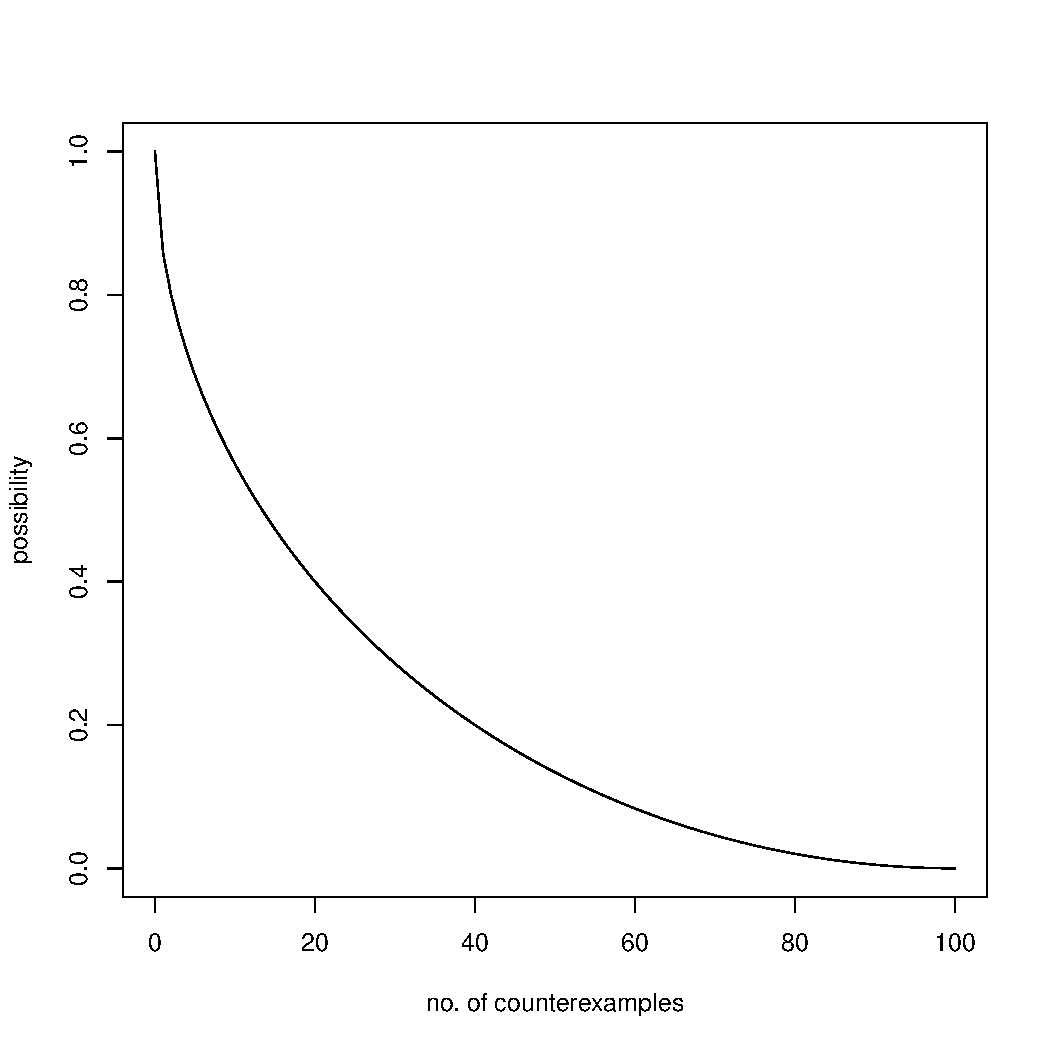
\includegraphics[width=1.4in]{../possibility} &
      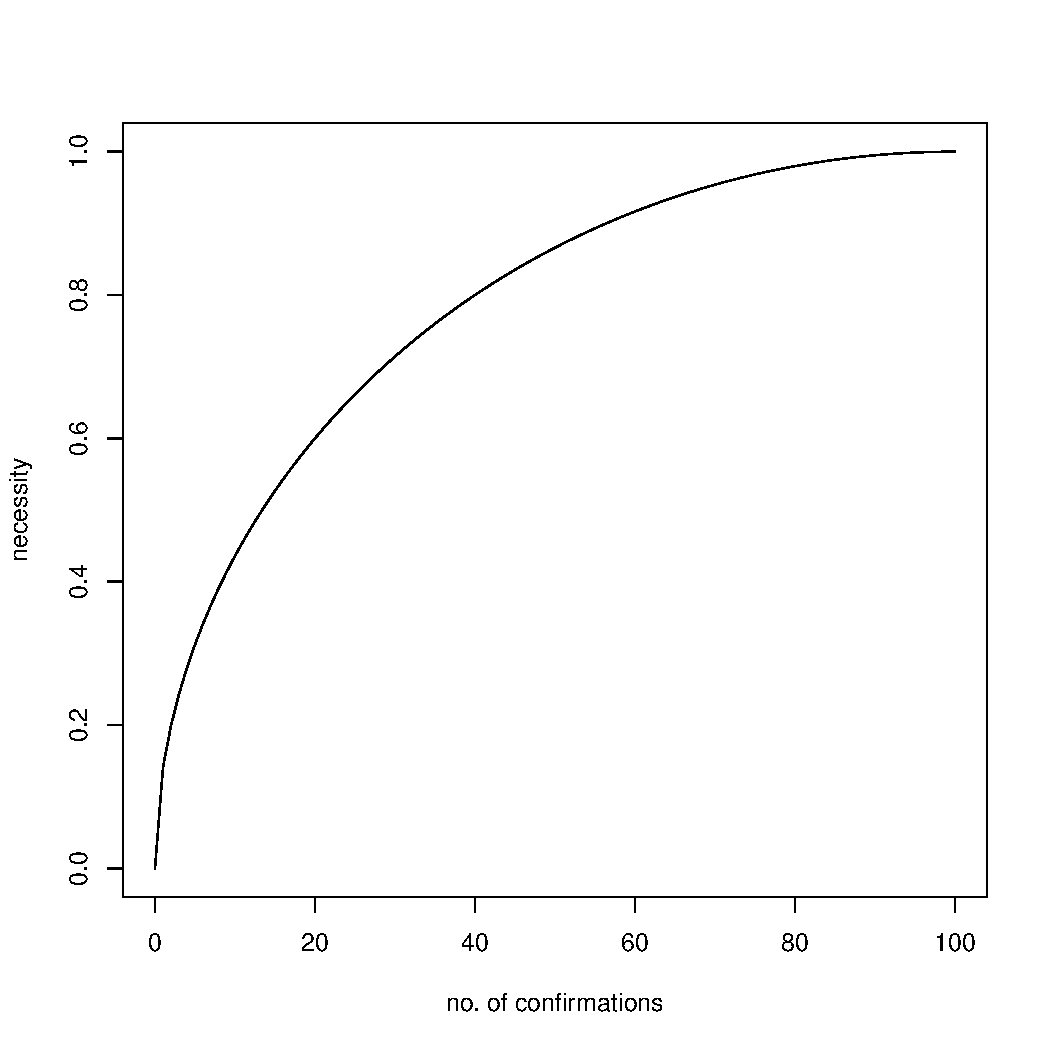
\includegraphics[width=1.4in]{../necessity}
    \end{tabular}
  \end{center}
}

\frame{\frametitle{Acceptance/Rejection Index}
  Combination of possibility and necessity of an axiom:
  \begin{definition}
    \[
      \mathrm{ARI}(\phi) = N(\phi) - N(\neg\phi) = N(\phi) + \Pi(\phi) - 1
    \]
  \end{definition}
  \begin{itemize}
  \item $-1 \leq \mathrm{ARI}(\phi) \leq 1$ for all axiom $\phi$
  \item $\mathrm{ARI}(\phi)<0$ suggests rejection of $\phi$ ($\Pi(\phi)<1$)
  \item $\mathrm{ARI}(\phi)>0$ suggests acceptance of $\phi$ ($N(\phi)>0$)
  \item $\mathrm{ARI}(\phi)\approx0$ reflects ignorance about the status of $\phi$
  \end{itemize}
}

\section{Candidate Axiom Testing}
\subsection[]{}

\frame{\frametitle{OWL~2 $\to$ SPARQL}
To test axioms, we define a mapping $Q(E, x)$ from OWL~2 expressions to SPARQL graph patterns
such that
\begin{center}
\texttt{SELECT DISTINCT ?x WHERE \{} $Q(E, \mbox{\tt ?x})$ \texttt{\}}
\end{center}
returns $[Q(E, x)]$, all known instances of class expression $E$
and
\[
  \mbox{\tt ASK \{ } Q(E, a) \mbox{\tt\ \}}
\]
checks whether $E(a)$ is in the RDF base.

\vfill
  \begin{exampleblock}{For an atomic concept $A$ (a valid IRI),}
    \[
      Q(A, \mbox{\tt ?x}) = \mbox{\tt ?x a }A\mbox{\tt~.}
    \]
  \end{exampleblock}
}

\subsection[]{Concept Negation}

\frame{\frametitle{Concept Negation: $Q(\neg C, \mbox{\tt ?x})$}

\begin{alertblock}{Problem}
  Open-world hypothesis, but no $\neg$ in RDF!
\end{alertblock}

We approximate an open-world semantics as follows:

  \begin{exampleblock}{}\vspace{-0.5em}
    \begin{equation}\label{eq:approx-open-world-negation}
      Q(\neg C, \mbox{\tt ?x}) =
      \begin{minipage}[t]{5in}
        \begin{tabbing}
          \quad\=\quad\=\quad\=\kill
          \{\>\texttt{?x a ?dc .}\\
            \>\texttt{FILTER NOT EXISTS} \{\\
            \>\>\texttt{?z a ?dc . } $Q(C, \mbox{\tt ?z})$\ \}\\
          \}
        \end{tabbing}
      \end{minipage}
    \end{equation}
  \end{exampleblock}

For an atomic class expression $A$, this becomes
  \begin{exampleblock}{}\vspace{-0.5em}
\begin{equation}
Q(\neg A, \mbox{\tt ?x}) =
  \begin{minipage}[t]{3in}
    \begin{tabbing}
      \quad\=\quad\=\quad\=\kill
      \{\>\texttt{?x a ?dc .}\\
        \>\texttt{FILTER NOT EXISTS} \{\\
        \>\>\texttt{?z a ?dc . ?z a} $A$ \} \}.
    \end{tabbing}
  \end{minipage}
\end{equation}
  \end{exampleblock}

}

%\frame{\frametitle{Concept Negation: Discussion}
%  \begin{center}
%    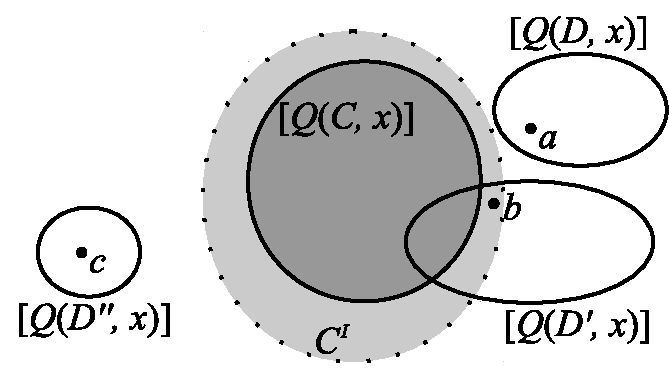
\includegraphics[height=2in]{../negation}
%  \end{center}
%}

\section{Subsumption Axiom Testing}
\subsection[]{}

\frame{\frametitle{$\mathsf{SubClassOf}(C\ D)$ Axioms}
  To test \textsf{SubClassOf} axioms, we must define their logical content
  based on their OWL~2 semantics:
\begin{eqnarray*}
  (C \sqsubseteq D)^\mathcal{I} &=& C^\mathcal{I} \subseteq D^\mathcal{I} \\
  &\equiv& \forall x\quad x \in C^\mathcal{I} \Rightarrow x \in D^\mathcal{I}
\end{eqnarray*}

Therefore, following the principle of selective confirmation,
\begin{block}{}
\[
  u_{C \sqsubseteq D} = \| \{D(a) : \mathcal{K} \models C(a) \} \|,
\]
\end{block}
because, if $C(a)$ holds,
\[
  C(a) \Rightarrow D(a) \equiv \neg C(a) \lor D(a) \equiv \bot \lor D(a) \equiv D(a)
\]
}

\frame{\frametitle{Support, Confirmations and Counterexamples of $C \sqsubseteq D$}
$u_{C \sqsubseteq D}$ can be computed by
\[
  \begin{minipage}[c]{5in}
    \begin{tabbing}
      \quad\=\quad\=\quad\=\kill
      \texttt{SELECT (count(DISTINCT ?x) AS ?u)}
      \texttt{WHERE} \{$Q(C, \mbox{\tt ?x})$\}.
    \end{tabbing}
  \end{minipage}
\]
As for the computational definition of $u^+_{C \sqsubseteq D}$ and $u^-_{C \sqsubseteq D}$:
\begin{itemize}
\item confirmations: $a$ s.t.\ $a \in [Q(C, x)]$ and $a \in [Q(D, x)]$;
\item counterexamples: $a$ s.t.\ $a \in [Q(C, x)]$ and $a \in [Q(\neg D, x)]$.
\end{itemize}
Therefore,
\begin{itemize}
\item $u^+_{C \sqsubseteq D}$ can be computed by
\[
  \begin{minipage}[c]{5in}
    \begin{tabbing}
      \quad\=\quad\=\quad\=\kill
      \texttt{SELECT (count(DISTINCT ?x) AS ?numConfirmations)}\\
      \texttt{WHERE} \{ $Q(C, \mbox{\tt ?x})$ $Q(D, \mbox{\tt ?x})$ \}
    \end{tabbing}
  \end{minipage}
\]
\item $u^-_{C \sqsubseteq D}$ can be computed by
\[
  \begin{minipage}[c]{5in}
    \begin{tabbing}
      \quad\=\quad\=\quad\=\kill
      \texttt{SELECT (count(DISTINCT ?x) AS ?numCounterexamples)}\\
      \texttt{WHERE} \{ $Q(C, \mbox{\tt ?x})$ $Q(\neg D, \mbox{\tt ?x})$ \}
    \end{tabbing}
  \end{minipage}
\]
\end{itemize}
}

\frame{\frametitle{Test a \texttt{SubClassOf} axiom (plain version, w/o time cap)}
\begin{algorithmic}[1]
  \REQUIRE $\phi$, an axiom of the form $\mbox{\tt SubClassOf}(C\ D)$;
  \ENSURE $\Pi(\phi)$, $N(\phi)$, confirmations, counterexamples.
  \STATE Compute $u_\phi$ using the corresponding SPARQL query;
  \STATE compute $u^+_\phi$ using the corresponding SPARQL query;
  \IF{$0 < u^+_\phi \leq 100$}
    \STATE query a list of confirmations;
  \ENDIF
  \IF{$u^+_\phi < u_\phi$}
    \STATE compute $u^-_\phi$ using the corresponding SPARQL query;\label{line:count-expt}
    \IF{$0 < u^-_\phi \leq 100$}
      \STATE query a list of counterexamples;
    \ENDIF
  \ELSE
    \STATE $u^-_\phi \leftarrow 0$;
  \ENDIF
  \STATE compute $\Pi(\phi)$ and $N(\phi)$ based on $u_\phi$, $u^+_\phi$, and $u^-_\phi$.
\end{algorithmic}
}

\frame{\frametitle{Comparison with a Probability-Based Score}
\vspace{-2em}
\begin{center}
  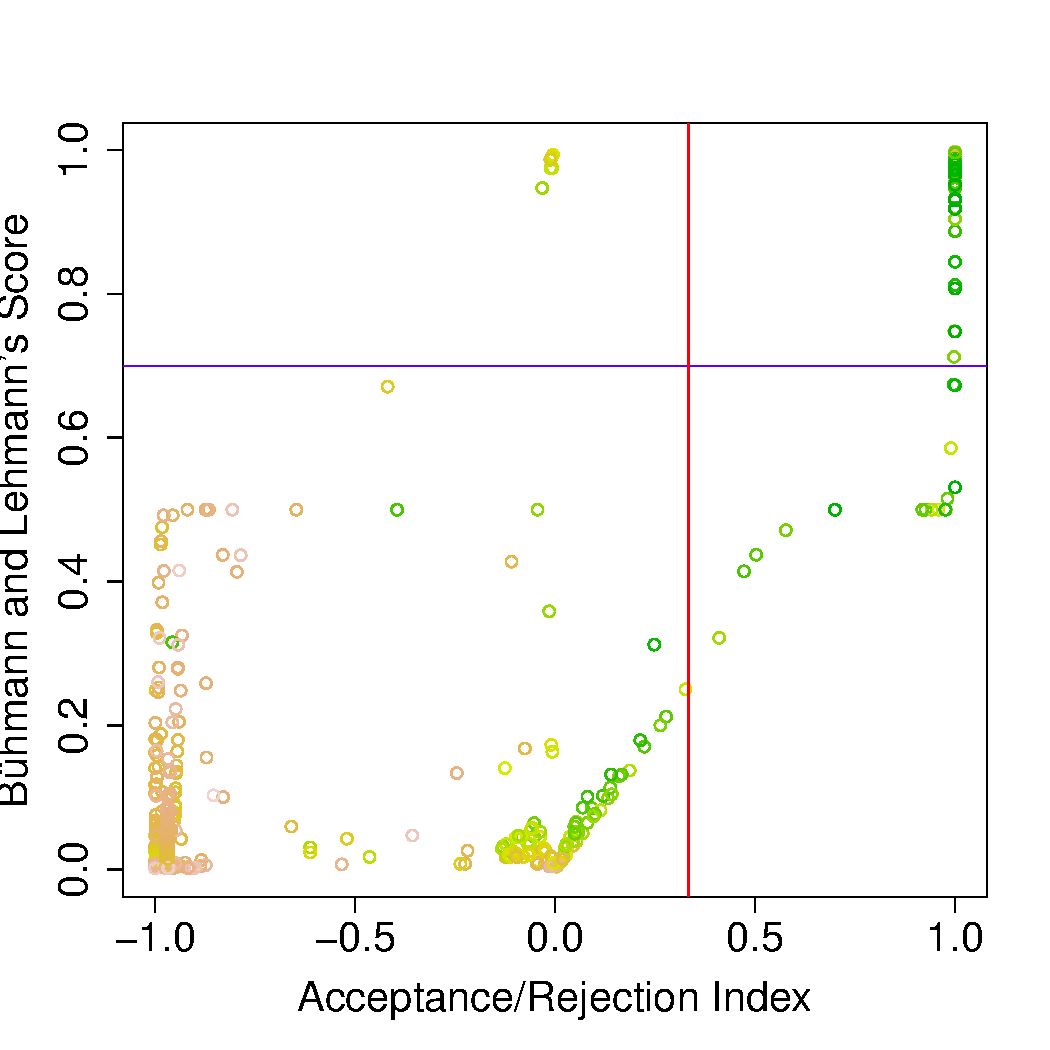
\includegraphics[height=3in]{ARI-BLS}
\end{center}
}

\subsection{Scalable Axiom Testing}

\frame{\frametitle{$T(\phi) = O\left((1 + \mathrm{ARI}(\phi))^{-1}\right)$
or $O\left(\exp(-\mathrm{ARI}(\phi))\right)$}
\vspace{-2em}
\begin{center}
  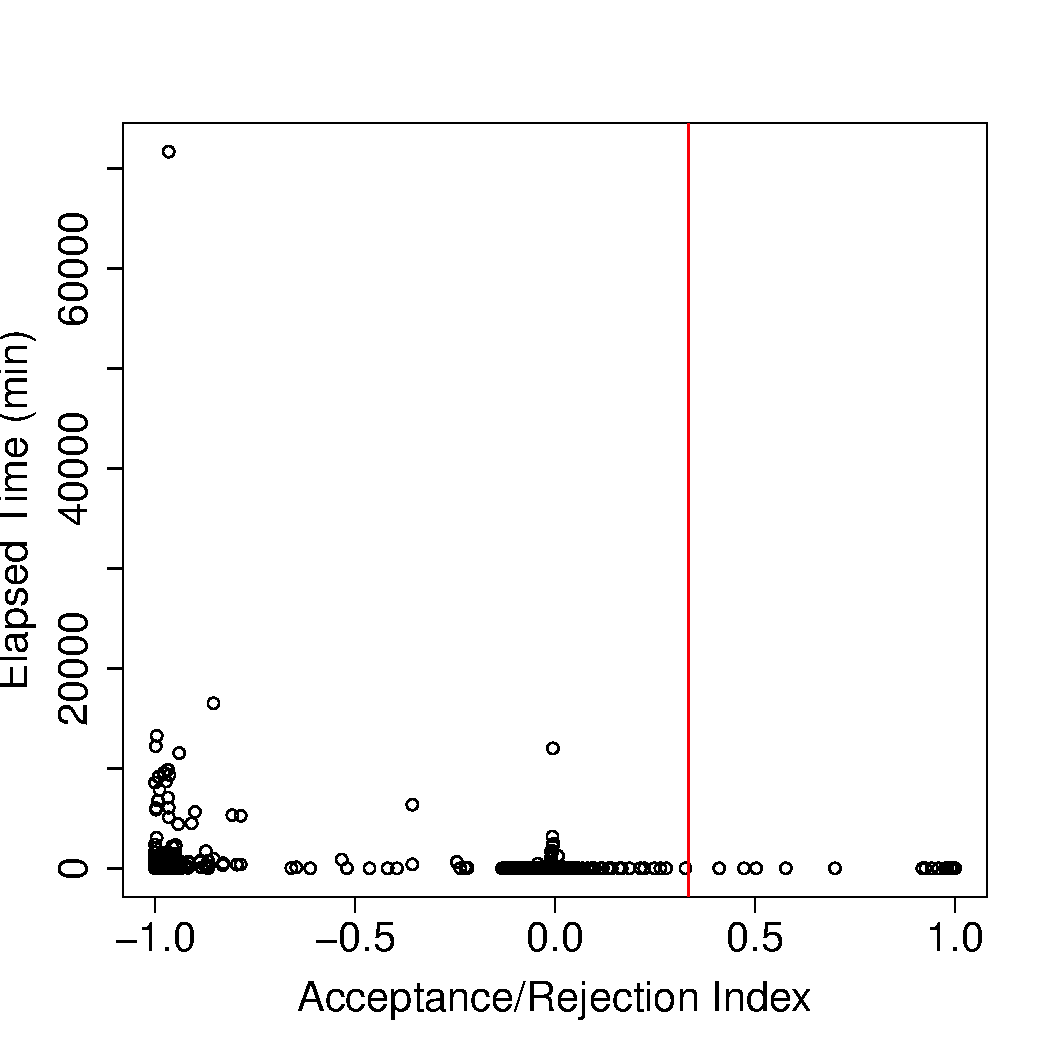
\includegraphics[height=3in]{time-ARI} 
\end{center}
}

\frame{\frametitle{Time Predictor}
\begin{alertblock}{}
How much time should we allow in order to be reasonably sure
we are not throwing the baby out with the bathwater, while avoiding to waste
time on hopeless tests?
\end{alertblock}
Studying the elapsed times for accepted axioms,
we observed that the time it takes to test $C \sqsubseteq D$ tends to be proportional to 
\[
  \mathrm{TP}(C \sqsubseteq D) = u_{C \sqsubseteq D} \cdot nic_C,
\]
where $nic_C$ denotes the number of intersecting classes of $C$. 

A computational definition of $nic_C$ is the following SPARQL query:
\begin{exampleblock}{}\vspace{-0.5em}
\[
  \begin{minipage}[c]{5in}
    \begin{tabbing}
      \quad\=\quad\=\quad\=\kill
      \texttt{SELECT (count(DISTINCT ?A) AS ?nic)}\\
      \texttt{WHERE} \{ $Q(C, \mbox{\tt ?x})$\quad \texttt{?x a ?A .} \}
    \end{tabbing}
  \end{minipage}
\]
\end{exampleblock}
where $A$ represents an atomic class expression.
}

\frame{\frametitle{$T(C \sqsubseteq D)/\mathrm{TP}(C \sqsubseteq D)$}
\vspace{-2em}
\begin{center}
  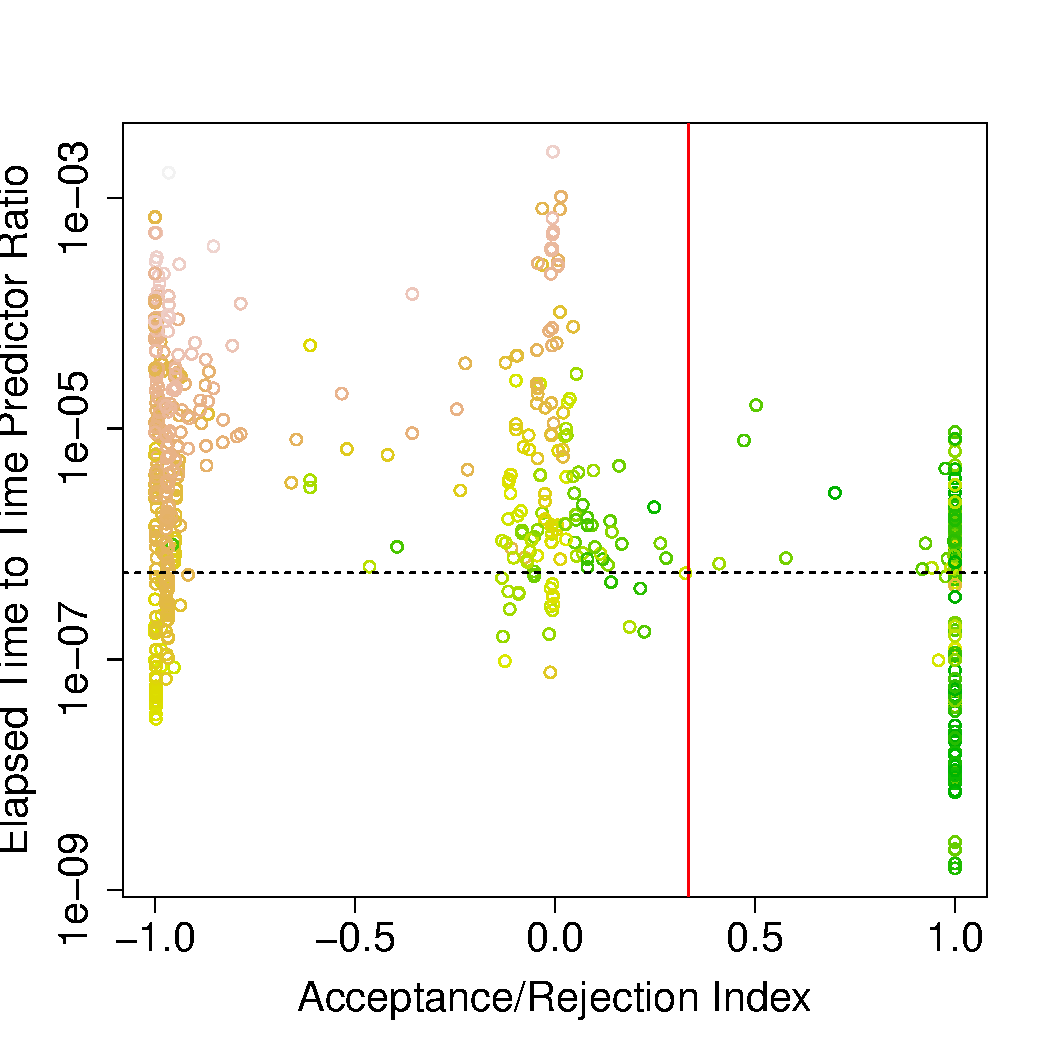
\includegraphics[height=3in]{ratio-ARI}
\end{center}
}

\frame{\frametitle{$\mathrm{TP}(C \sqsubseteq D)$ as a function of the cardinality rank of $C$}
\vspace{-2em}
\begin{center}
  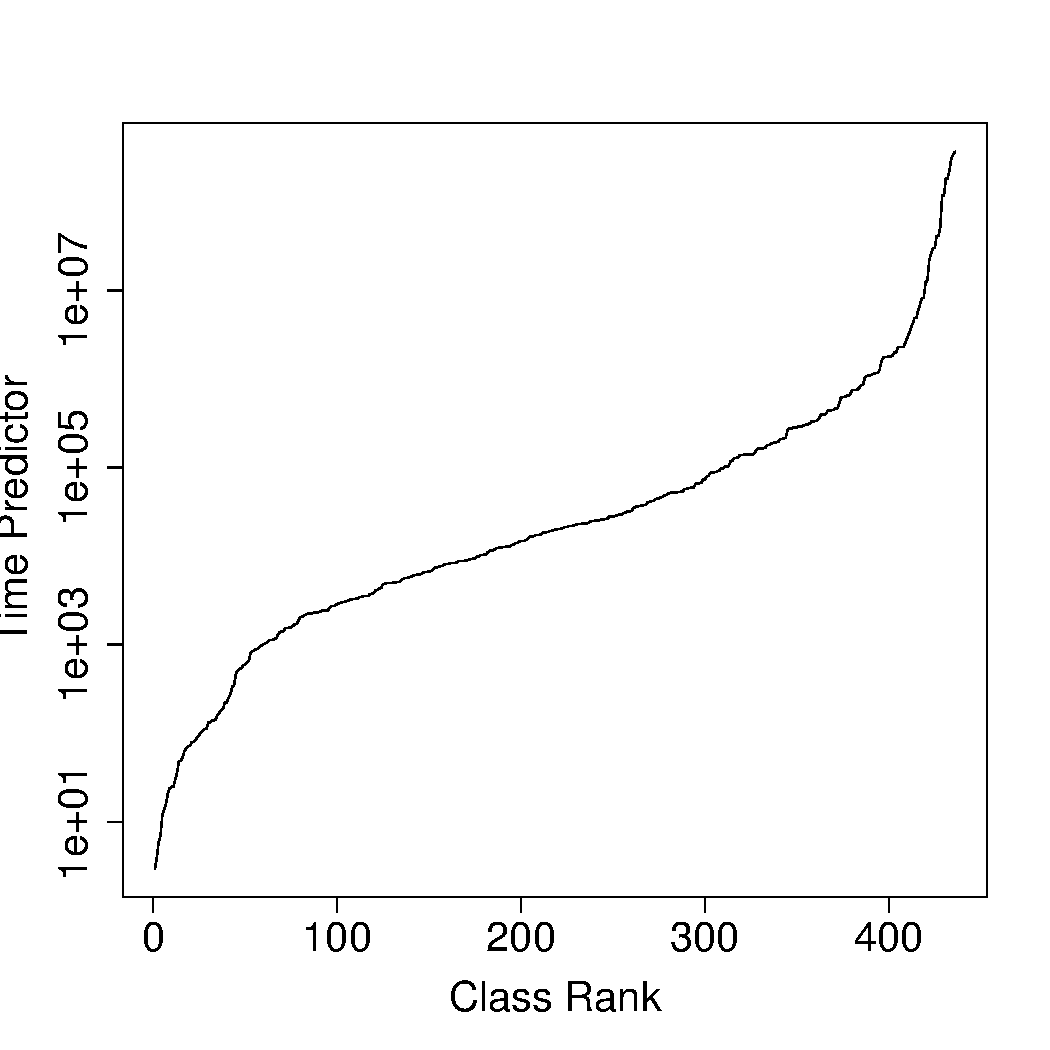
\includegraphics[height=3in]{tp}
\end{center}
}

\frame{\frametitle{Test a \texttt{SubClassOf} axiom (time-capped version)}
\renewcommand{\algorithmicfor}{\textbf{waiting up to}}
\begin{algorithmic}[1]\scriptsize
  \REQUIRE $\phi$, an axiom of the form $\mbox{\tt SubClassOf}(C\ D)$;\\
    $a$, $b$, the coefficients of the linear time cap equation.
  \ENSURE $\Pi(\phi)$, $N(\phi)$, confirmations, counterexamples.
  \STATE Compute $u_\phi$ and \VAR{nic} using the corresponding SPARQL queries;
  \STATE $\mathrm{TP}(\phi) \leftarrow u_\phi \cdot \VAR{nic}$;
  \STATE compute $u^+_\phi$ using the corresponding SPARQL query;
  \IF{$0 < u^+_\phi \leq 100$}
    \STATE query a list of confirmations;
  \ENDIF
  \IF{$u^+_\phi < u_\phi$}
    \STATE $t_{\max}(\phi) \leftarrow a + b\cdot\mathrm{TP}(\phi)$
    \FOR{$t_{\max}(\phi)$ min}
      \STATE compute $u^-_\phi$ using the corresponding SPARQL query;
    \ENDFOR
    \IF{\textbf{time-out}}
      \STATE $u^-_\phi \leftarrow u_\phi - u^+_\phi$;
    \ELSIF{$0 < u^-_\phi \leq 100$}
      \STATE query a list of counterexamples;
    \ENDIF
  \ELSE
    \STATE $u^-_\phi \leftarrow 0$;
  \ENDIF
  \STATE compute $\Pi(\phi)$ and $N(\phi)$ based on $u_\phi$, $u^+_\phi$, and $u^-_\phi$.
\end{algorithmic}
}

\section{Experiments}

\subsection[]{}

\frame{\frametitle{Experiments}
Experimental Setup:
\begin{itemize}
\item DBpedia 3.9 in English as RDF fact repository
\item Local dump (812,546,748 RDF triples) loaded into Jena TDB
\item Method coded in Java, using Jena ARQ and TDB
\item 12 6-core Intel Xeon CPUs @2.60GHz (15,360 KB cache),
128 GB RAM, 4 TB HD (128 GB SSD cache),
Ubuntu 64-bit OS.
\end{itemize}
Systematically generate and test SubClassOf axioms involving atomic classes only
\begin{itemize}
\item For each of the 442 classes $C$ referred to in the RDF store
\item Construct all $C \sqsubseteq D$ : $C$ and $D$ share at least one instance
\item Test these axioms in increasing time-predictor order
\item Compare with scores obtained w/o time cap
\end{itemize}
}

\subsection[]{}

\frame{\frametitle{Time-Capped Score vs. Probability-Based Score}
\vspace{-2em}
\begin{center}
  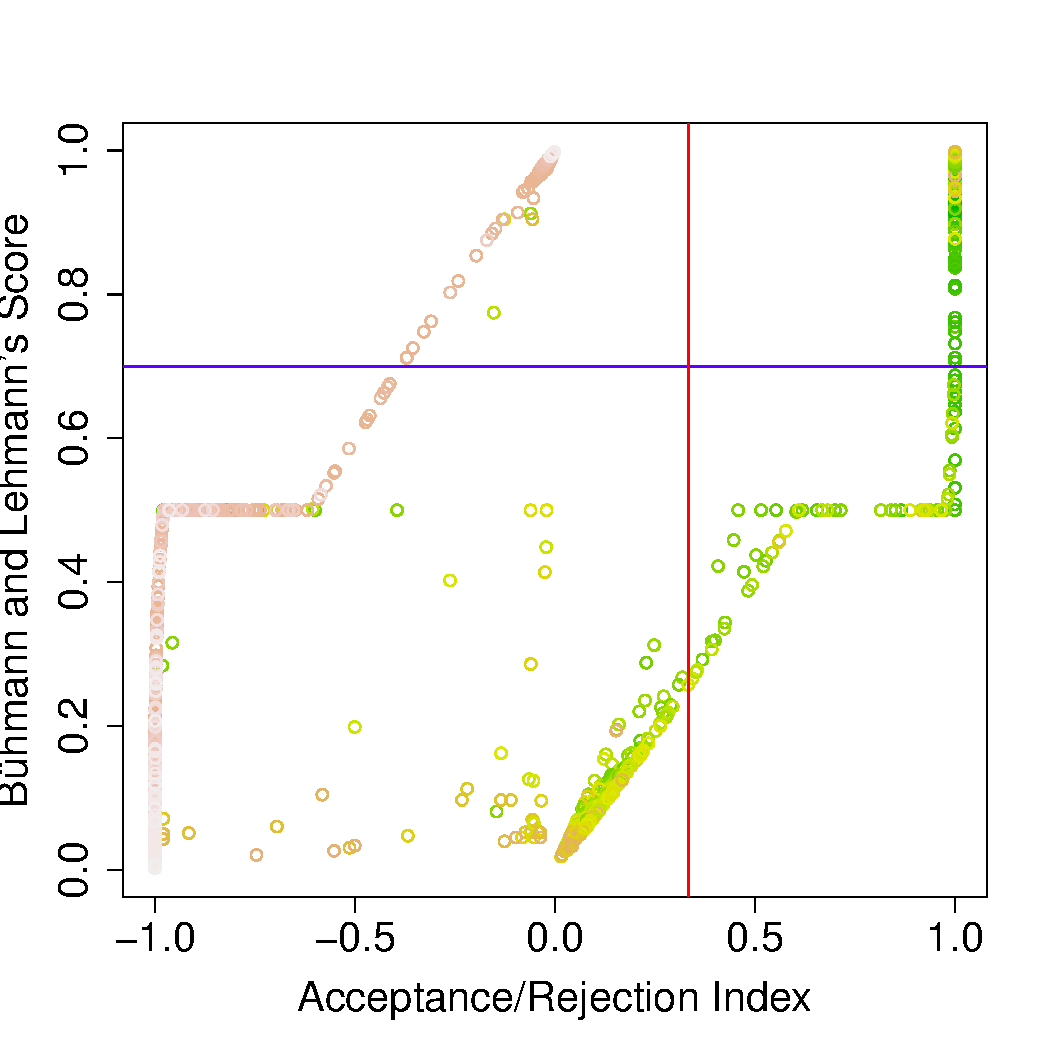
\includegraphics[height=3in]{ARI-BLS-dtc}
\end{center}
}

\frame{\frametitle{Results}
Speed-up:
\begin{itemize}
\item Testing 722 axioms w/o time cap took 290 days of cpu time
\item We managed to test 5,050 axioms in $<$ 342 h 30' (244 s/axiom) w/ time cap
\item 142-fold reduction in computing time
\end{itemize}

Precision loss due to time capping:
\begin{itemize}
\item 632 axioms were tested both w/ and w/o time cap
\item Outcome different on 25 of them: a 3.96\% error rate
\end{itemize}

Absolute accuracy:
\begin{itemize}
\item Comparison to a gold standard of DBpedia Ontology \texttt{SubClassOf} axioms
  + \texttt{SubClassOf} axioms that can be inferred from them
\item Of the 5,050 tested axioms, 1,915 occur in the gold standard
\item 327 (17\%) get an $\mathrm{ARI} < 1/3$
\item 34 (1.78\%) get an $\mathrm{ARI} < -1/3$
\end{itemize}
}

\section{Conclusion}
\subsection[]{}

\frame{\frametitle{Conclusions \& Future Work}

Contributions
\begin{itemize}
\item Axiom scoring heuristics based on possibility theory
\item A framework based on the proposed heuristics
\item Time capping to reduce the computational overhead
\end{itemize}

Results
\begin{itemize}
\item Experiments strongly support the validity of our hypothesis
\item 142-fold speed-up with $<$ 4\% increase of error rate
\item Human evaluation suggests most axioms accepted by mistake
  are inverted subsumptions or involve ill-defined concepts
\end{itemize}

Future work
\begin{itemize}
\item Extend experimental evaluation to other types of axioms
\item Enlarge test base w/ additional RDF datasets from the LOD
\end{itemize}
}

\frame{\frametitle{The End}
  \makenote{\huge Thank you for your attention!}
}

\end{document}
